\chapter{Methods}\label{chapter2}
\section{Selecting an approach}\label{sec:selecting_an_approach}
To begin developing a solution to the super-resolution (SR) reconstruction problem in remote sensing, we must select an approach that will enable us to produce a solution in-line with our goals and within project scope. There are two approaches to select from to achieve this: either designing and implementing an entirely novel solution, or further developing a pre-existing one. A completely novel solution provides opportunity to produce state-of-the-art SR reconstructions but requires expert domain knowledge and an extensive time-frame for in-depth solution development. Further developing a pre-existing solution may only allow for incremental improvements when compared to a novel, state-of-the-art solution, however the strong developmental foundation and documentation of common challenges permits more efficient solution development.

The complexity of recently proposed solutions to the SR reconstruction problem in remote sensing surpasses the scope of this project due to the composition of network architectures, dataset sizes, hardware requirements etc. To produce a novel solution we would be required to extend beyond recent developments, causing the novel approach to be out of scope for this project. Therefore, iterating upon a pre-existing solution is the approach we will select.

In section~\ref{sec:background_research} we explored a variety of solutions to the SR reconstruction problem in remote sensing, providing several candidate solutions for us to choose from. The super-resolution generative adversarial network (SRGAN)~\cite{srgan}, proposed by Ledig \etal\ in 2017 is a generalised solution to the SR reconstruction problem. Being the first generative adversarial network (GAN) based SR reconstruction solution, the model provides a desirable set of characteristics for additional development. Firstly, the model is well established within the field of SR reconstruction resulting in numerous public implementation repositories that we may use as reference points for our implementation, reducing the time spent logic debugging. SRGAN also has the benefit of a lightweight solution architecture when compared to recent solutions, which would lead to faster training times, allowing us to test a larger variety of adaptations. Another benefit of the lightweight architecture is that it would be able straightforward to introduce adaptations to the model. 

The main argument against selecting SRGAN as our foundation is that it is no longer state-of-the-art when compared to newer solutions. The issue with selecting a newer foundation is that we may encounter implementation difficulties due to the lack of publicly available guidance from previous implementations. Additionally, the potential for incremental improvement on recent solutions becomes limited due to their complex nature. Further, it is relatively easy to identify two areas of SRGAN that can be improved to produce greater SR reconstruction capabilities on remote sensing imagery. Firstly, SRGAN is a generalised SR reconstruction model and is trained on a non-specific dataset. By training SRGAN on a remote sensing dataset we will achieve better SR reconstructions when applying the model to remote sensing imagery. Secondly, a key component of the loss function, perceptual loss, utilises the pretrained VGG19~\cite{vgg19} model to calculate the `perceptual' difference between training data and model outputs~\cite{srgan}. This perceptual loss value guides SRGAN towards producing better results, however the VGG19 component is outdated, with numerous potential replacements for us to explore. Given the arguments explored above, and the easily identified solution improvements, we will use SRGAN as the foundation for our solution.

\section{Tools and practices}
The following section explores tools and best practices to ensure effective solution development, whilst providing justification for the tools and practices we choose to adopt.

\subsection{Tools}
SRGAN is a type of neural network, meaning we will need to implement a neural network architecture for our solution.\ \code{Python} is programming language extensively used for data-related purposes and in the field of machine learning. It provides a high level interface for a variety of common processes that we can utilise in the development of our solution. An alternative choice is \code{C++}, a low-level programming language designed for tasks where efficiency is crucial. Using \code{C++} to implement the solution would result improved efficiency over \code{Python}, but would introduce significantly more development time and a steeper learning curve, as it requires the developer to manage significantly more features than \code{Python} does. We will use \code{Python} as the programming language for our solution due to its ease of use over \code{C++}.

Accompanying \code{Python} are a plethora of libraries we may use to simplify and enhance the development of our solution. An important choice is the library we will use for neural network development, to avoid doubling efforts where implementations already exist. There are two main neural network libraries, \code{TensorFlow}~\cite{tensorflow} and \code{PyTorch}~\cite{pytorch}, each providing interfaces for the creation of neural networks in \code{Python}. Both provide very similar functions, such as network implementation, steepest gradient descent, preprocessing etc. Either library is sufficient for our implementation, however there exists an alternative that simplifies the development process even further.\ \code{Keras}~\cite{keras} is another neural network library that acts an interface to more complex libraries \code{TensorFlow}, \code{PyTorch} or \code{Jax}. It simplifies the entire development process, whilst also retaining functionality for implementing more complex features, where the complexity is hidden from the developer until access is necessary for solution development. We will use \code{Keras} for the development of our solution due to its simplicity. The default backend library is \code{TensorFlow}, which we will maintain as the \code{Keras} documentation often references \code{TensorFlow}'s documentation directly.

Additional \code{Python} libraries include \code{NumPy} for numerical operations and \code{Matplotlib} for visualisation purposes. Both libraries are used extensively across \code{Python} applications and are accompanied by exhaustive documentation. We will use these over the alternatives due to their widespread adoption and in-depth documentation.

\subsection{Practices}
Ensuring stable and efficient development of the solution requires employing development best practices. Version control is a practice used to maintain a history across the entire span of development, promoting healthy development processes. Using version control when developing the solution ensures a timeline of progress, useful for project management, rectifying incorrect changes and producing proof of solution development.\ \code{Git} is widely used version control software that tracks changes to files within a repository, enabling easy version control with a few simple commands.\ \code{Git} is considered the industry standard for version control and is widely documented, therefore we will use it for the development of the solution.

There are also considerations for the code that we write as a part of this project. Maintaining clean, modular code ensures minimal time wasted on traversing and understanding messy code whilst debugging. We will ensure that each aspect of the implementation is sufficiently modular, where related functions are grouped together in the same \code{Python} files. Functions more closely associated will be grouped with \code{Python} classes. The result is reusable, modular code that enables effective development. To keep our implementation code readable, we will make use of documentation and comments where necessary. These allow for a greater understanding of functionality beyond reading the code line-by-line and aids code reuse. 

Alternatively, \code{Jupyter} notebooks may be used.\ \code{Jupyter} provides a `notebook' style of development where related sections of code can be separated into cells and ran independently. Functionality to write and style documentation within the notebook is also available.\ \code{Jupyter} is an excellent choice for many machine learning projects and is widely used to implement solutions across the industry, however it struggles to deal with large amounts of data and complex programs, commonly resulting in software crashes. As a result we will implement well-documented, modular code in standard \code{Python} files.

\section{Data}
The following section explores the available datasets and justifies our selection.

\subsection{Datasets}
GANs require training data to learn from. In the case of SR reconstruction, training data is composed of pairs of images: a high-resolution (HR) and low-resolution (LR) version of each training instance. During training time, the model will learn a generalised mapping between the two resolutions, which can then be applied to unseen LR imagery to generate an SR result. As identified in section~\ref{sec:selecting_an_approach}, SRGAN is trained on a non-specific dataset which may resulting in less-desirable results when applying SRGAN to remote sensing imagery. Therefore, to ensure the best possible results for our solution we will train SRGAN on remote sensing imagery. A series of remote sensing image datasets have been widely accepted by the community as effective at training learning-based SR reconstruction methods. Wang et al.~\cite{remoteSensingDeepLearningReview, remoteSensingGANsReview} overview such datasets in two papers exploring deep learning-based SR reconstruction solutions.
\begin{table}
    \centering
    \begin{tabular}{cccc}
        \toprule
        \textbf{Name} & \textbf{Size} & \textbf{Resolution} & \textbf{File type} \\
        \midrule
        AID & 10000 & 600 $\times$ 600 & JPG \\
        RSSCN7 & 2800 & 400 $\times$ 400 & JPG \\
        WHU-RS19 & 1005 & 600 $\times$ 600 & TIF \\
        UC Merced & 2100 & 256 $\times$ 256 & PNG \\
        NWPU-RESISC45 & 31500 & 256 $\times$ 256 & PNG \\
        RSC11 & 1232 & 512 $\times$ 512 & TIF \\
        UCAS-AOD & 910 & 1280 $\times$ 659 & PNG \\
        SIRI-WHU & 2400 & 200 $\times$ 200 & TIF \\
        ITCUD & 135 & 5616 $\times$ 3744 & JPG \\
        DIOR & 23463 & 800 $\times$ 800 & JPG \\
        DOTA & 2806 & 800 $\times$ 4000 & PNG \\
        \bottomrule
    \end{tabular}
    \caption{Table of remote sensing datasets commonly used for SR reconstruction as suggested by Wang et al.~\cite{remoteSensingDeepLearningReview,remoteSensingGANsReview}.}
    \label{table:datasets_table}
\end{table}

The selection of dataset must be in line with our project goals. We aim to pick the most diverse dataset whilst ahering to the limitations introduced to us by training hardware. To avoid large training times the resolution of the images must not be too large, but also not so small that we are unable to learn any meaningful mappings between LR and HR. The dataset must also be of a sufficient size, as a dataset that is too small will result in unsatisfactory training results. Having a large dataset is acceptable as we are able to reduce the number of training images down based on hardware limiations.

Following these requirements removes the WHU-RS19, UCAS-AOD, and ITCUD datasets for having too few images, along with DOTA for having too large of a resolution. This yields the AID, RSSCN7, UC Merced, NWPU-RESISC45, RSC11, SIRI-WHU and DIOR datasets. Any of these datasets would prove effective for training SRGAN.

Notably, the NWPU-RESISC45 dataset contains the most images and the most image classes, providing opportunity for SRGAN to learn from a greater variety of remote sensing images and produce better generalisation when applied to unseen imagery. The dataset is also accompanied by a pre-built data loader as a part of the \code{Tensorflow Datasets}~\cite{tensorflowDatasets} \code{Python} library, making loading and processing the data convenient and efficient. Training with all 31500 images is impossible with the hardware available to us, so taking a subset of the dataset is necessary to ensure we do not encounter out-of-memory errors. The large size of the dataset also means we may split our selection into training, validation and testing sets without affect size of the training set, which could result in reduced learning capabilities. As the NWPU-RESISC45 dataset provides some minor benefits over the other available datasets, especially the pre-built data loader, we will select it as the dataset for SRGAN training, validation, and testing. 

\subsection{NWPU-RESISC45 dataset}\label{subsec:resisc45}
The Northwestern Polytechnical University REmote Sensing Image Scene Classification dataset consists of 31500 remote sensing images gathered from Google Earth~\cite{resisc45}. The dataset boasts 45 unique image classes, allowing us to introduce a wide variety of image to SRGAN during training time. Additionally, images are sampled with a lare variety of characteristics, inluding translation, spatial resolution, viewpoint, object pose, illumination etc~\cite{resisc45}.
\begin{figure}
    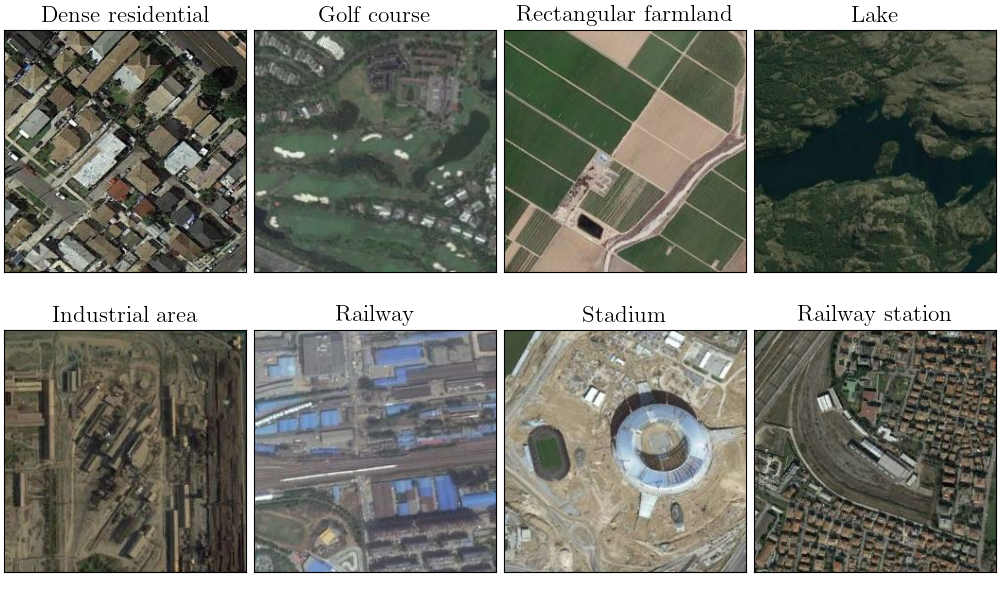
\includegraphics[width=\linewidth]{./assets/resisc45_example.png}
    \caption{Some example images from the training subset of the NWPU-RESISC45 dataset.}
    \label{fig:resisc45_examples}
\end{figure}

\subsection{Data preparation}\label{subsec:data_preparation}
Before we can train SRGAN to produce SR reconstructions we must prepare the data it will learn from. The first step is to split the dataset into three distinct sets: training, validation and testing sets, where SRGAN learns how to reconstruct images from the training set, the validation set is used to measure performance during training time, and the testing set is used to measure final model performance. It is crucial to have these as distinct sets to appropriately evaluate the effectiveness of our solution. For example, testing model performance on the training set after training time generates inaccurate performance metrics as the model has been exposed to the images beforehand. Similarly, validating model performance on the training set alone during training time creates biased performance metrics.

Before deciding the sizes of the training, validation and testing sets, we must consider the stratification of the dataset. Stratification ensures that each of the image classes within the dataset are proportionally represented when taking subsets. This is crucial, as having unproportional image classes within the dataset results in unproportional SR reconstruction capabilities. If SRGAN recieves more training instances of, for example, images with the classification `Lake', then the final trained model may be better at reconstructing lakes but worse at reconstructing images from other classes. As our dataset contains 45 classes, with each class containing exactly 700 instances, we must ensure that each of our training, validation and testing sets contains an equal number of images from each class. The size of each set must therefore be a multiple of 45.

The size of the each of the training, validation and testing sets is primarily decided by the hardware limitations imposed by the machines that the solution is trained on. As a result, we cover the justification for the size of each of the sets in section~\ref{subsec:procedure}. Conducting tests into the dataset size limit yields a final training set size of $n = 945$. Keeping in line with the common practice of a ratio of 80\%:10\%:10\% for training, validation and test set sizes, we yield validation and testing sets of sizes $n = 135$ to ensure each of our sets are properly stratified.

To learn how to create SR reconstructions, SRGAN requries LR and HR pairs of images so that it may learn the mapping between the two. NWPU-RESISC45 provides us with the HR imagery, however we still need LR imagery for training. As described by Ledig \etal, the HR imagery is downsampled using a bicubic kernel with $r = 4$ to produce the LR imagery~\cite{srgan}. To prepare our LR images we followed this process, however encountered unsatisfactory results in the form of artefacts appearing in the downsampled outputs. Conducting further research revealed that using a bicubic kernel for image downsampling has the potential to produce artefacts due to anti-aliasing, a technique employed to reduce sharp edges in images~\cite{antialiasing}. To solve this issue, the imagery can first be blurred before downsampled~\cite{blurring, srgan}, which reduces the requirement for anti-aliasing and avoids creating artefacts. Image blurring is executed using a Gaussian kernel of size $3 \times 3$. Introducing the blurring step successuly removed the anti-aliasing artefacts.

\section{Solution}
In the following section we provide a detail on SRGAN, the foundation of our solution to the SR reconstruction problem in remote sensing. We adapt the loss function of a pre-existing model by systematically testing model performance with different loss variations. Details of the implementation are presented.

\subsection{Architecture}\label{subsec:architecture}
The architecture of the solution is provided by the SRGAN model proposed by Ledig et al.\ in 2017. The SRGAN architecture follows the typical generative adversarial network architecture~\cite{gan}, consisting of a generator and a discriminator. The role of the generator is to produce SR reconstructions, and the discriminator aids in guiding the generator towards producing a desirable result through adversarial training.

The generator of SRGAN is designed to extract features and then upsample the input image. It does this through a series of so-called `residual blocks'. Residual block network architectures employ skip connections to reintroduce features from previous layers back into the activations following later convolutions~\cite{residualNets}. This ensures that information captured in previous layers does not get degraded when passing through a deep network architecture~\cite{residualNets}. Each of the residual blocks consists of five layers, where each layer executes some operation on the output of the previous layer. First the image is passed through a convolution layer to extract image features. Next a batch normalisation (BN) layer is executed on the output from the convolutional layer to centre and rescale the values. Batch normalisation ensures standardisation of model values and promotes accelerated, stable training~\cite{batchNorm}. The output from the BN layer is passed through a parametric ReLU (PReLU) layer where the activations of the neurons are calculated. PReLU acts the same as a normal ReLU layer, but the parameters of the ReLU function are also learned during training time to allow for complex non-linearity to be harnessed. The PReLU layer is followed by another convolutional and batch normalisation pair to further extract image features and then normalise. Finally, the output of the block is added to the input value to enact the skip connection function. The model architecture consists of $n$ of these residual blocks. The residual block portion of the architecture is followed by two upsampling blocks. These blocks consist of a convolutional layer, followed by a pixel shuffle layer and finally a PReLU activation layer. Each upsample block upsamples by a factor of two, so introducing two blocks creates an upsampling factor of four. Following the upsample layers is a single convolutional layer designed to reshape the feature maps into a $W \times H \times C$ format, which we can represent as an image. After model training this output resembles the LR input image upsampled by a factor of four. It is important to note that Ledig \etal propose the generator component as a standalone model named SRResNet, using mean squared error as the loss component. As suggested by Ledig \etal , we use a pretrained SRResNet model as the initial generator component of SRGAN. Specific training functionality is detailed in the following section.

The discriminator follows a standard binary classifier architecture. Images are passed through several convolutional blocks that capture the image features and then downsample. Following these blocks is a fully connected layer that reduces the number of neurons down to one, where the activation of the final neuron decides the classification of the image. In the case of a GAN, a classification of 0 or False represents a real image, and classification of 1 or True represents a fake image constructed by the generator. 

\begin{figure}
    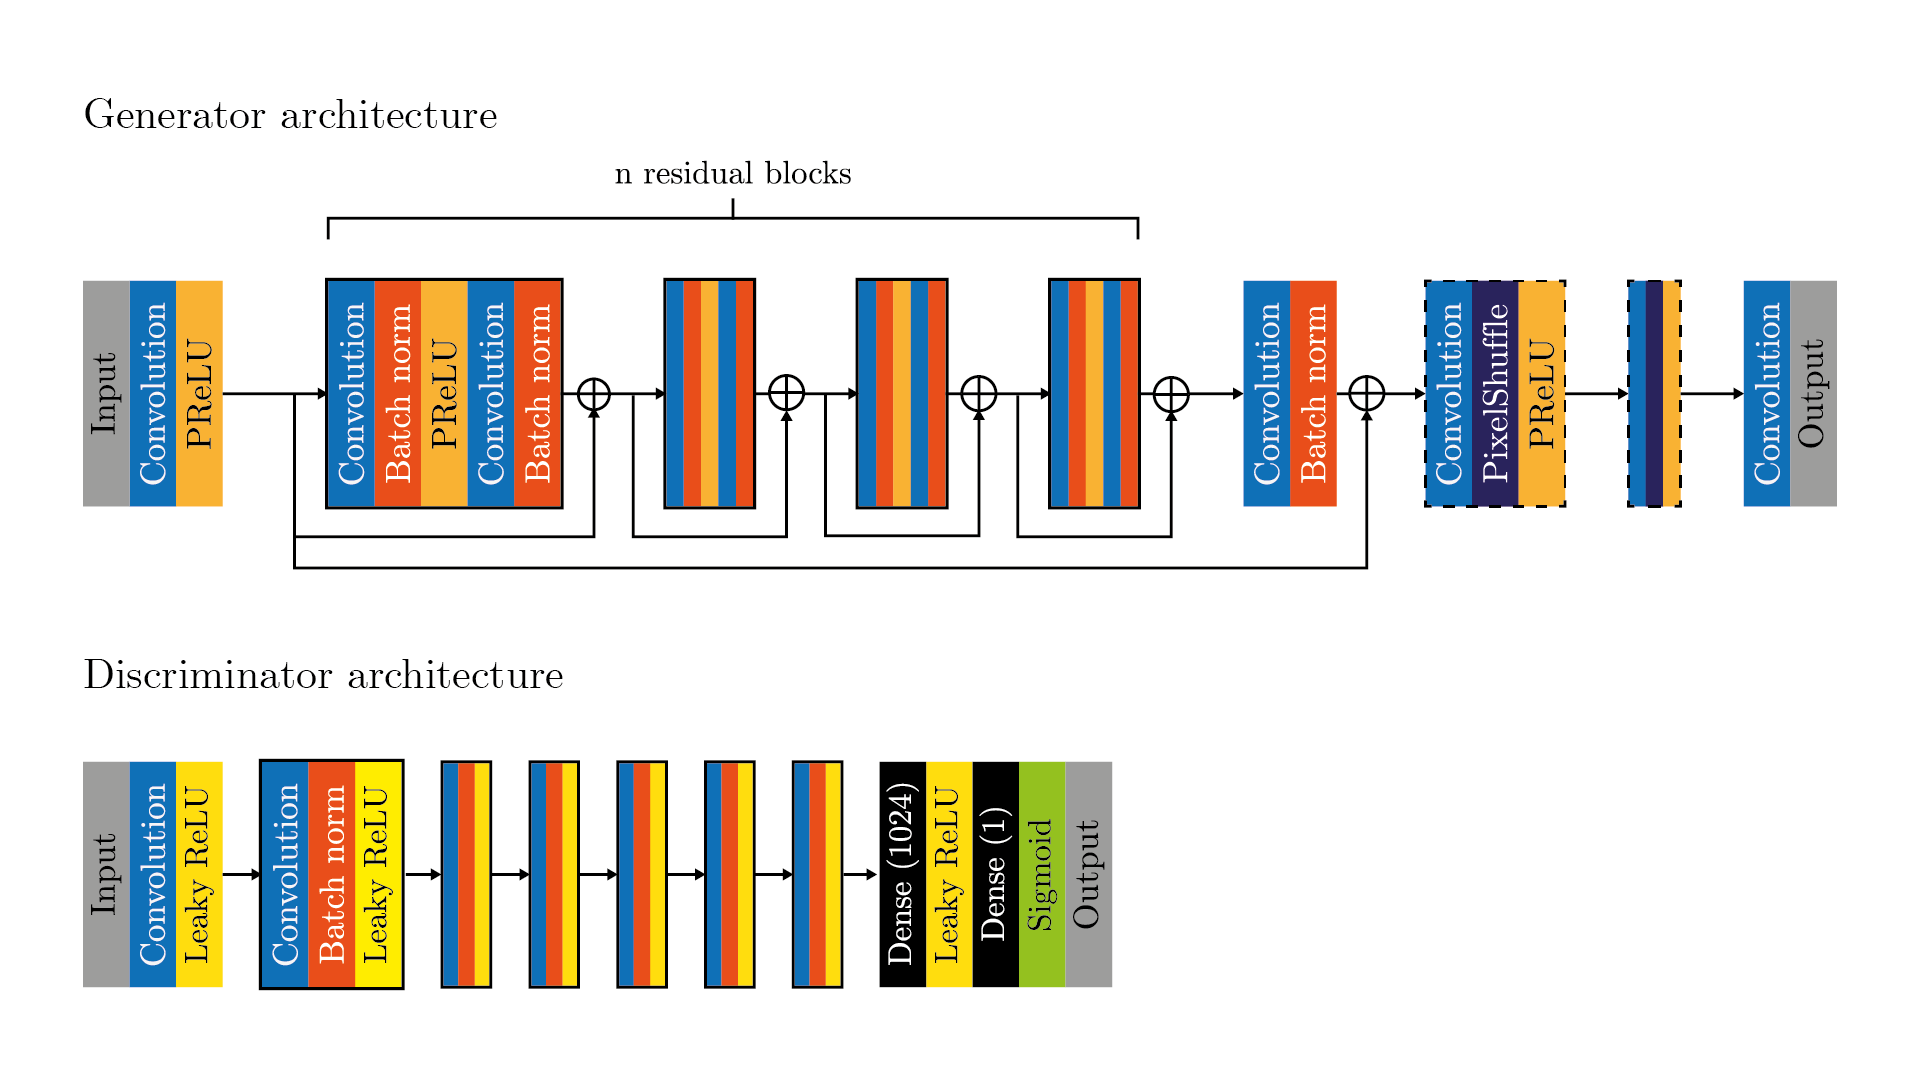
\includegraphics[width=\linewidth]{./assets/srgan_architecture.png}
    \caption{An image illustrating the layer architecture of both the generator and discriminator components of SRGAN.}
    \label{fig:srgan_architecture}
\end{figure}

\subsection{Training functionality}\label{subsec:training_functionality}
Providing LR imagery to the solution architecture prior to training will result in SR reconstructions resembling random noise due to initialising the model with random weights. To produce good SR reconstructions we must train SRGAN on our training dataset, so it can learn a generalised mapping between LR and HR imagery.

Prior to training SRGAN we must first pretrain the generator, as suggested by Ledig \etal \ to reduce the likelihood of undesirable local optima~\cite{srgan}. For each training step, LR imagery is generated by downsampling HR images. We pass the LR imagery through the model to create the SR reconstructions, and calculate training loss by computing the pixel-wise mean squared error (MSE) between the HR images and SR reconstructions. Steepest gradient descent is used to calculate how to adust the model weights to produce a lower MSE and consequently better SR reconstruction capabilities.

Ledig \etal \ provide description of the SRGAN training process. Each training step consists of two parts: generator training and discriminator training. Firstly the discriminator is trained. We take the input HR imagery and downsample using the method described in section~\ref{subsec:data_preparation} to produce corresponding LR imagery. The LR imagery is fed into the generator component in its current state to produce SR reconstructions. HR and SR images are then concatenated and corresponding image labels are created, with a label of 0 for HR imagery and a label of 1 for SR imagery. Next, the concatenated images and their corresponding labels are fed into the discriminator component, which will predict image labels for each of the training instances. The binary cross-entropy loss is calculated between the actual and predicted image labels to give a value representing the `distance' the discriminator needs to traverse to achieve more accurate classifications. Gradient descent with the Adam optimiser is used to calculate how to nudge the model parameters to produce a lower binary cross-entropy loss value, which in turn produces more correct classifications.

Generator training follows discriminator training. Firstly we take the same LR and HR images used for discriminator training, and again pass the LR images to the generator component to create SR reconstructions. We then generate `misleading' image labels for the SR reconstructions, essentially labelling the SR reconstructions as HR instead. We pass the SR reconstructions and the misleading labels to the discriminator to predict fake and real labels for each reconstruction. We then calculate the binary cross-entropy loss between the misleading labels and the discriminator predictions. This achieves the effect of producing a value representing how well our generator has `fooled' the discriminator into thinking the SR reconstructions are HR imagery. This loss value is called the adversarial loss component. The next step is to calculate the perceptual loss component. To do this, both the HR imagery and SR reconstructions are passed through our perceptual loss model, which Ledig \etal \ introduce as the high-level feature maps produces by the VGG19 model. The mean squared error is then calculated between the HR and SR feature maps to provide a `perceptual distance' between the HR imagery and our SR reconstructions. Minimising this value creates SR reconstructions with a greater perceptual similarity to the corresponding HR image. The perceptual loss is added to the adversarial loss, with the adversarial loss being scaled by a value of $10^{-3}$ as suggested by Ledig \etal \ We then use steepest gradient descent to calculate how to change our model weights to produce an overall lower generator loss (the combined adversarial and perceptual loss) using the Adam optimiser.

\subsection{Improving loss}\label{subsec:improving_loss}
Ledig \etal \ utilise a pretrained VGG19 model to produce feature maps for the both the generated SR image and the HR ground truth. The pixel-wise mean squared error of the feature maps is calculated to provide a scalar value representing the perceptual difference between the two images, which acts as a component of the training loss. The VGG19 model is trained to classify images, so the learned feature maps produce the highest classification accuracy possible, in turn identifying the most important and distinctive features of each image class. By calculating the difference between these feature maps we can see how much the most important features in the SR reconstruction differ from the ground-truth image, and point the model towards a result with greater realism.

We can extend this idea to image classification models that outperform VGG19. A superior classification accuracy suggests the model has better extracted the most important image features~\cite{featureExtraction}. We can utilise such models as replacements for the VGG19 component of the perceptual loss. We offer the following conjecture: `using the feature maps from more accurate image classification models in the perceptual loss component of SRGAN-based models will increase SR reconstruction performance'.

To explore this, with the aim of producing a solution to the SR reconstruction in remote sensing, we  test model performance using feature maps from a variety of pretrained image classification models. The \code{Keras} library provides numerous image classifiers pretrained on the ImageNet database. Within the documentation for these pretrained classifiers are accuracy metrics, calculated on the ImageNet validation dataset, allowing us to select models based on their performance. The available classifiers can be grouped into classes based on their model architecture, allowing us to select the model with the highest accuracy from each class as the perceptual loss component for SRGAN training. A full list of available models can be found in Appendix~\ref{appendix}.

Calculating the loss with a pretrained model requires a minor alteration to the model architecture to be feasible. The models consist of convolutional sections followed by fully-connected layers of neurons, where the activations of the final layer of neurons represent the `certainty' that the image belongs to each class. We are not interested in the classification of our images, but rather the distinct image features, thus we remove the fully connected layers of neurons from each model leaving the desired feature maps. When calculating loss during training time, both the HR image and the SR reconstruction are passed through the model and the image feature maps are created. The pixel wise mean squared error is calculated between the feature maps, and the resulting value is the loss for that training step. Minimising this value produces better SR results.

\begin{table}
    \centering
    \begin{tabular}{ccccc}
        \toprule
        \textbf{Classifier} & \textbf{Top-1 accuracy} & \textbf{Top-5 accuracy} & \textbf{Size (MB)} & \textbf{Parameters (M)} \\
        \midrule
        Xception & 79.0\% & 94.5\% & 88 & 22.9 \\
        ResNet152V2 & 77.2\% & 94.2\% & 232 & 60.4 \\
        InceptionV3 & 77.9\% & 93.7\% & 92 & 23.9 \\
        InceptionResNetV2 & 80.3 \% & 95.3\% & 215 & 55.9 \\
        MobileNetV2 & 71.3\% & 90.1\% & \textbf{12} & \textbf{3.5} \\
        DenseNet201 & 77.3\% & 93.6\% & 80 & 20.2 \\
        NASNetLarge & 82.5\% & 96.0\% & 343 & 88.9 \\
    EfficientNetV2L & \textbf{85.7\%} & \textbf{97.5\%} & 479 & 119.0 \\
        \bottomrule
    \end{tabular}
    \caption{List of pretrained image classifiers tested as the perceptual loss component for SRGAN training. The best value in each category is highlighted in green.}
    \label{table:pretrained_classifiers}
\end{table}

For each of the pretrained classifiers an SRGAN model was trained using the classifier feature maps to calculate the perceptual loss. The training procedure used for the SRGAN models is described in section~\ref{subsec:procedure}.

\subsection{Implementation}
The model architecture and training functionality was implemented in \code{Python} primarily using the \code{Keras} library.\ \code{Keras} provides interfaces for implementing neural network applications and enables the implementation of the solution architecture as described in section~\ref{subsec:architecture}. Creating a machine learning model is as simple as instantiating and ordering \code{Keras} classes that represent neural network layers. Following the model definition we can compile it with the appropriate loss and optimiser and expose it to training data.\ \code{Keras} then handles the low-level training operations such as steepest gradient descent, backpropagation etc. The final model weights can be saved for performance testing and future use.

The above approach works well for simple neural networks that do not require much customisation, however this will not be sufficient for building SRGAN due to the complex training functionality as described in section~\ref{subsec:training_functionality}. Thankfully \code{Keras} provides the option to expose lower-level features of the library, effectively allowing us to take control of the training procedures and implement our own functionality. This is achieved through subclassing the \code{keras.Model} class and overriding the training step. Much of the customisation in \code{Keras} works this way, where library classes are subclassed and required methods are overridden. We will first implement SRResNet as its own class, where we define the model architecture and the training functionality. This allows us to independently define and train SRResNet, ready to be used as the initial generator model for SRGAN training. We take the same approach for the SRGAN model, where we define the network architecture using the \code{keras} interface. We then override the training step and implement the SRGAN training functionality. Whilst implementing the SRGAN model we use documentation from Keras and an external source to aid us when debugging logic issues~\cite{keras, srganImplementation}.

In addition to overriding the training step we override the test step. At the end of each epoch a validation test is executed where the model is validated on unseen imagery. For the test step the loss is calculated on the input imagery the same as the respective SRResNet and SRGAN train steps, with the difference being that the loss is not used to influence the model weights. Instead, the validation loss is used to identify the configuration of model weights that produce the best SR reconstructions.

Accompanying the model implementations are various \code{Python} files, designed to offer support to the model definition and training process. These include definitions of custom layers where \code{Keras} does not offer functionality, custom losses as described in section~\ref{subsec:improving_loss}, data loading interfaces, training execution, and general utilities. A full list of \code{Python} files and their contributions to the implemntation are listed in apendix~\ref{ref}.

\section{Training}
The following section describes and justifies the procedure used to train the SR reconstruction models.

\subsection{Existing guidance}
Ledig et al.~\cite{srgan} provide in-depth detail on how they trained the SRResNet and SRGAN models to achieve high-quality SR results. Both models were trained on a 350000 image subset of the ImageNet database~\cite{imageNet}. 16 sub-image patches of size $96 \times 96$ are taken of distinct training images. The Adam~\cite{adamOptimiser} optimiser is used with $\beta_1 = 0.9$. The SRResNet model is trained on the dataset for a total of $10^6$ update iterations using a learning rate of $10^{-4}$. The SRGAN model is trained for $10^5$ update iterations with an initial learning rate of $10^{-4}$, followed by another $10^5$ update iterations using a learning rate of $10^{-5}$. To avoid unwanted local optima the pretrained SRResNet is used as the generator for the SRGAN model.

\subsection{Procedure}\label{subsec:procedure}
Training the SRResNet and SRGAN models from scratch will require a deviation from existing training guidance to account for time and hardware limitations. This section outlines the exact training procedure that was followed along with justification for the differences to the original procedure as defined by Ledig et al.~\cite{srgan}.

The guidance regarding the randomly cropped sub-images used to train the model is unclear. The exact guidance states `For each mini-batch we crop 16 random $96 \times 96$ HR sub images of distinct training images'. This could be interpreted in two ways: either a batch consists of 16 images and a single $96 \times 96$ patch is taken from each image in the batch, or, a batch has an undefined size, but for every image in the batch 16 random patches of size $96 \times 96$ are taken to increase the training set size, known as data augmentation~\cite{dataAugmentation}. For the purposes of this project we assume the second definition to be true as it allows us to introduce more training examples to the model through data augmentation to hopefully improve final performance.

Taking the sub-images definition as described above requires us to choose an appropriate batch size. Choosing a batch size requires balancing model results and memory constraints~\cite{batchSizeTest}. A larger batch size produces a smoother gradient to traverse but also requires significantly more memory and computation resources. Alongside this, we also need to consider a batch size that nicely factors into our dataset size. Picking a dataset size, batch size and number of patches required an investigation into the memory limitations introduced by the training hardware. The number of image classes in the NWPU-RESISC45 dataset is considered first. There are 45 distinct image classes, as listed in section~\ref{subsec:resisc45}. To avoid unintentionally overfitting our SR reconstruction model to a specific class we must include an equal number of images from each of the 45 classes, consequently requiring our dataset size to be a multiple of 45. Therefore, it is also required that the batch size factors into 45 to ensure that the entire dataset is visited over a single epoch and no training examples are skipped due to division remainders. 

A larger batch size produces a smoother gradient and therefore more stable training, however the hardware available restricts how large the batch size can be. Employing a method of trial and error identifies a batch size suitable for training the SR reconstruction model whilst adhering to memory constraints. A sample dataset of size 450 is used to test different batch sizes, with the intention of later increasing the dataset size to increase training examples. Firstly, training of the SRGAN model begins with a batch size and a single image patch per training example. The system attempts to allocate the required memory resources and computing power from the GPU but is unable to, resulting in an out-of-memory (OOM) exception. The batch size is then reduced, and the process is repeated until no OOM exception occurs. In practice the first batch size selected was $b = 30$, which resulted in an OOM exception. This value was reduced until a final batch size of $b = 15$ was selected. The next step was to test the memory constraints on the number of patches taken from each training example. A similar approach was taken to selecting batch size, where the number of patches was reduced until running model training no longer yielded an OOM exception. The initial value was $p = 16$, as suggested by Ledig et al., with the test yielding $p = 10$ patches per training instance. Further testing showed that for $p = 10$ and $p = 9$ that training would begin but that halt at seemingly random points in the process. To combat this, the number of patches was further reduced to $p = 8$, which yielded no OOM exceptions. Finally, the dataset size was selected by employing the same trial and error approach, where a dataset size of $n = 945$ was yielded. The final sizes are a batch size of $b = 15$, number of patches $p = 10$ and dataset size $n = 945$. Specific details on how the dataset subset was generated can be found in section~\ref{subsec:data_preparation}. We can also calculate the number of epochs and the number of steps per epoch (update iterations). An epoch step is defined as model training for one batch. Each image only appears once across all batches, meaning our total number of steps per epoch is:
\[\frac{\textnormal{Dataset size}}{\textnormal{Batch size}} = \frac{945}{15} = 63\]
Following the calculation of the steps per epoch, we are able to calculate the number of epochs required for $10^5$ and $10^4$ update iterations:
\[\Bigg\lceil\frac{10^5}{\textnormal{Steps per epoch}}\Bigg\rceil = \Bigg\lceil\frac{10^5}{63}\Bigg\rceil = 1588\]
\[\Bigg\lceil\frac{10^4}{\textnormal{Steps per epoch}}\Bigg\rceil = \Bigg\lceil\frac{10^4}{63}\Bigg\rceil = 159\]
The selection of batch size, dataset size and number of patches allows for remaining training details to be considered. As suggested by Ledig et al.\ the Adam optimiser is used with $\beta_1 = 0.9$, the SRResNet model is trained with a learning rate of $10^{-4}$, the initial training for the SRGAN model is trained with a learning rate of $10^{-4}$, and the fine-tuning training is executed with a learning rate of $10^{-5}$. The pretrained SRResNet model is used as the initial generator of the SRGAN model to reduce the likelihood of undesirable local optima~\cite{srgan}. The Ledig et al.\ procedure suggests $10^6$ update iterations for the pretrained SRResNet model. With the available training hardware and batch size, dataset size and number of patches training would take $\sim$48 hours. Due to the University of Leeds machines restarting every day, training the model for that long becomes tricky. As a result of this it makes sense to reduce the number of update iterations to $10^{5}$, reducing the training time to just over four hours. In interest of maintaining the guidance set out by Ledig et al.\ the number of update iterations for the first pass and fine-tune training of the SRGAN model should also be reduced by a factor of 10 to be proportional, yielding $10^4$ update iterations. Figure~\ref{table:model_training} provides a summary of the training parameters for all training scenarios.
\begin{table}
    \centering
    \begin{tabular}{cccc}
        \toprule
        {} & \textbf{SRResNet} & \textbf{SRGAN 1\textsuperscript{st} pass} & \textbf{SRGAN 2\textsuperscript{nd} pass} \\
        \midrule
        \textbf{Batch size} & 15 & 15 & 15\\ 
        \textbf{Patches} & 8 & 8 & 8 \\
        \textbf{Dataset size} & 945 & 945 & 945\\
        \textbf{Adam $\beta_1$} & 0.9 & 0.9 & 0.9\\
        \textbf{Learning rate} & $10^{-4}$ & $10^{-4}$ & $10^{-5}$ \\
        \textbf{Update iterations} & $10^5$ & $10^4$ & $10^4$ \\
        \textbf{Epochs} & 1588 & 159 & 159 \\
        \textbf{Steps per epoch} & 63 & 63 & 63 \\
        \bottomrule
    \end{tabular}
    \caption{Summary of the details and parameters used for model training.}
    \label{table:model_training}
\end{table}

At the end of each epoch, or one training cycle through the entire dataset, the model performance is validated using the validation set. As described in section~\ref{subsec:data_preparation}, 135 images, or three images for each of the 45 classes present in the NWPU-RESISC45 dataset compose the validation set. On epoch end, the validation images are processed (blurred and downsampled), and then fed through the SR reconstruction model. The losses are then calculated the same as they would be for each training step. A final validation loss is produced, which tells us how well the model performs on unseen remote sensing imagery as training proceeds. Once this loss is calculated at the end of every epoch, it is compared to the `best' or lowest validation loss that the model has produced in training. If the validation loss from the most recent epoch is lower than the previous best validation loss, then the current state of the model is saved, replacing the previous best state. This process repeats until model training is completed. The final saved model state will therefore be the state that produced the lowest loss when applied to unseen imagery, or the state of the model with the best SR reconstruction capabilities. The saved model states can then be loaded and applied to more imagery or trained further. They can be found within the project repository.